\chapter{Geometric Vortex Pinning}
\label{theoryvortex}

\section{London Superconductivity}
Superconductivity was first explained throught he light of Maxwell's equations. In 1935, Fritz and Heinz London used their equations to explain the Meissner effect. these can be derived from Ampere's law:
\begin{eqnarray}
\nabla \times \overrightarrow B  = \mu_0 \overrightarrow J,
\label{Ampere}
\end{eqnarray}
where $\overrightarrow B$ is the magnetic field, $\mu_0$ is the permeability of free space, and $\overrightarrow J$ is the current. We then use the vector identity

\begin{eqnarray}
\nabla \times \nabla \times \overrightarrow A  = -\nabla^2 \overrightarrow A,
\label{stokes}
\end{eqnarray}
to get
\begin{eqnarray}
\nabla^2 B = \frac{B}{\lambda_p^2},
\label{penetration}
\end{eqnarray}

where $\lambda_p$ is the penetration depth. While these equations were good at describing the macroscopic properties of superconductors, better theories such as the Langevin system had to be derived to describe vortices. 

\section{Langevin system for vortices}
The Langevin system for vortices is a relatively simple place to start. It keeps only vortex degrees of freedom and foregoes all other perturbations of the complex order parameter. As long as the pinning centers are not too dense and vortices stay further appart than their coherence length, this provides a fairly accurate system. Looking at the equation of motion for this overdamped system, one can get an idea of the forces involved:
\begin{eqnarray}
\eta \frac {\partial u}{\partial t} = \epsilon_1 \frac {\partial^2 u} {\partial z^2 } + \Sigma_j F_{vp} (u - R) \delta(z - z_j) + j + F_T(z,t), 
\label{Langevin}
\end{eqnarray}
where $\eta$ is the viscosity coefficient, $\epsilon$ is the line tension, $f$ is the current's driving force, $(R,Z)$ are the random pinning coordinates, $F_{vp}$ is the pinning force, and $F_T$ is the thermal randomizing force. From this equation, one can see that the current driving force is trying to push overdamped vortices through a viscous fluid. Every once in a while, they get stuck in pinning centers and may or may not get out again depending on the current force and the thermal noise. Finally if the system is in 3 dimensions, then the vortices will want to stay in as straight of a line as possible~\cite{Kwok16}. As simple and intuitive as the Langevin system may be, it falls short on explaining other important phenomena such as vortex creation, cutting, and reconnection. Also, it cannot explain phenomena related to $T_C$ variation. For these we need a much more powerful system called the time dependent Ginzburg Landau model. 

\section{The Ginzburg-Landau Model for Superconductivity}
Superconductivity near the transition temperature can be succinctly characterized by a complex order parameter field $\psi$. Near this critical temperature, the free energy of the system becomes
\begin{eqnarray}
F = F_n + \alpha |\psi|^2 + \frac {\beta} {2} |\psi|^4 + \frac {1} {2m} |(-i \hbar \nabla - 2 e \overrightarrow A) \psi|^2 + \frac {|\overrightarrow B |^2} {2 \mu_0}
\label{freeE}
\end{eqnarray}
where $F_n$ is the free energy, $\alpha$ and $\beta$ are system constants which will be defined later,$\mu_0$ is the magnetic permeability of free space , $m$ is the cooper pair effective mass, $e$ is electron charge, $\overrightarrow A$ is the magnetic vector potential, and $\overrightarrow B$ is the magnetic field. Being interested in the physical reprecussions of this kind of system, we minimize the free energy with respect to the order parameter and vector potential to get

\begin{eqnarray}
\alpha \psi + \beta |\psi|^2 \psi + \frac {1} {2m} (-i \hbar \nabla - 2 e \overrightarrow A)^2 \psi = 0
\label{GLEQ1}
\end{eqnarray}
\begin{eqnarray}
\nabla \times \overrightarrow B = \mu_0 \overrightarrow j
\label{GLEQ2}
\end{eqnarray}
\begin{eqnarray}
\overrightarrow j = \frac {2e} {m} Re(\psi^* (-i \hbar \nabla - 2 e \overrightarrow A) \psi)
\label{GLEQ3}
\end{eqnarray}
where $j$ is the current and $Re$ is the real part. Equation ~\ref{GLEQ1} can be thought of in two parts. The first part ($\alpha \psi + \beta |\psi|^2 \psi $) is just the component relating to the superconductor, without supercurrent. Above the superconducting temperature, only $\psi = 0$ solves the equation. Below the superconducting temperature we have $|\psi|^2 = -\frac {\alpha} {beta}$, which is reminiscent of a quantum observable. The second half of ~\ref{GLEQ1} is basically a modified version of the Schrodinger time-independent equation, but with a magnetic potential. ~\ref{GLEQ2} is Ampere's law. ~\ref{GLEQ3} is also similar to a quantum observable with $ -i \hbar \nabla - 2e \overrightarrow A$ as the momentum operator in the presence of a magnetic field. The Ginzburg-Landau equations can be related to the microscopic Bardeen-Cooper-Schrieffer theory ~\cite{Sadovskyy14}. 

The SciDAC project revolves around a program called {\sc GLGPU} which models the important parameter function $\psi$ using the time dependent Ginzburg Landau equations:
\begin{eqnarray}
\Gamma (\partial_t +i \frac{2e}{\hbar}\mu)\psi = a_0 \epsilon (r) \psi - b |\psi|^2 \psi + \frac{1}{4m} (\hbar \Delta + \frac{2e}{ic} A)^2 \psi + \xi (r,t)
\label{TDGL1}
\end{eqnarray}
and
\begin{eqnarray}
\kappa^2 \nabla \times (\nabla \times A) = J_n + J_s + I,
\label{TDGL2}
\end{eqnarray}
where $u = \Gamma/(a_0 t_0)$, $t_0$ is the unit of time, and $J$ is the total current density. This program models a discretized system which is initialized with a parameter function and then each timestep is defined by following the TDGL equation. Using this program, we studied many situations such as grids of non-superconducting inclusions, funnels, vortex ratchets, and critical currents.


\section{Large $\lambda$ Limit}
The surface of a superconducting field is a rich interplay between the coherence length $\xi = \sqrt{\hbar^2/4ma_o}$ and the magnetic penetration length $\lambda = \sqrt{mc^2 / 8\pi e^2 \psi^2_0}$, where $\psi = \sqrt{a_0/b_0}$ is the equilibrium value of the order parameter in the absence of an electromagnetic field. The ratio $\chi = \lambda / \xi$ is called the GL parameter. 

 In high temperature superconductors, the penetration length $\lambda$ is typically much larger than the coherence length $\xi$. One consequence of this is that at length scales smaller than $\lambda$, the magnetic field is basically constant. The coherence length comes from the fermi velocity for the material and the energy gap between conducting and superconducting states~\cite{Kittel96}.  $\xi$ describes the length over which the superconducting electron density can change. This is also the size to which a cooper pair can spread. Another place it comes in is determining the size of the core of the vortex. 

\section{Phenomenological Vortex Interactions}

\subsection{Vortex-Vortex Interactions}
	 Vortex flux lines will move due to Lorentz forces $W = d \cdot F = d \cdot (B \times I)$ where $W$ is the energy drained away by moving vortices, $d$ is the distance the vortex travels, $F$ is the force on the vortex, $B$ is the field of the vortex, and $I$ is the current of the system. Whether or not a vortex will move is complicated and hard to study analytically. There are many factors which affect the movement of a vortex. First, vortices which rotate in the same direction will push each other away~\ref{sameV}. Conversely, if the vortices spin in the same direction, they will attract and annihilate each other~\ref{diffV}. This can be explained if one looks at the lorentz forces of a vortex-vortex system.

\begin{figure}[htbp]
\begin{center}
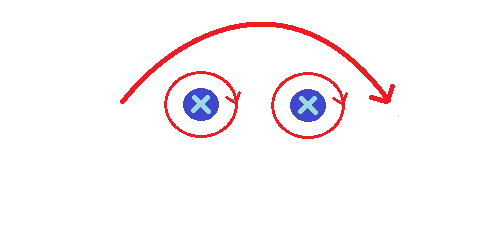
\includegraphics[scale=.50]{sameDirection.png}
\caption{The right hand rule tells us which direction the currents will swirl around a vortex pointing into the page. Then using Lorentz's law  at the second vortex, we can see that the second vortex will be pushed away. The same thing is happening from the current of the second vortex onto the first. Another way to see it is that in between the two vortices, the induced currents are cancelled out. Meanwhile on the outside of the vortices, the induced current adds up. The vortices will then feel a force which pushes them away from each other.}
\label{sameV}
\end{center}
\end{figure}

\begin{figure}[htbp]
\begin{center}
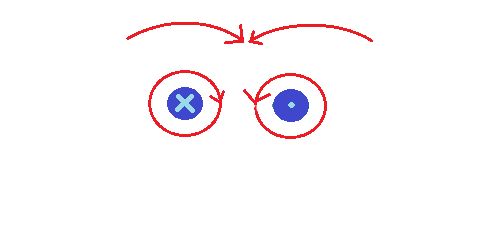
\includegraphics[scale=.50]{oppositeDirection.png}
\caption{The right hand rule tells us which direction the currents will swirl around a vortex pointing into the page. Then using Lorentz's law  at the second vortex, we can see that the second vortex will be pulled in this time. The same thing is happening from the current of the second vortex onto the first (although the second current flows in the opposite direction). In this case, the induced current between the vortices adds up while the current on the outsides cancels out. This makes the vortices move towards each other.}
\label{diffV}
\end{center}
\end{figure}

\subsection{Vortex-Defect Interactions}
The interaction between vortices and defects have been well-studied. Defects can be used to pin vortices and reduce dissipation. Defects can be impurities, vacancies, and inclusions. In one dimension they can be defects such as dislocations and irradiation tracks. Finally in three dimensions, they can be twin boundaries or stacking faults. The structure of atomic defects can have scattering properties which are either potential or magnetic type. Cooper pair-breaking caused by these defects has the effect of lowering the critical temperature. While studying these is important for pinning dynamics, it is the defecs which are on the order of several coherence lengths which are of interest to us. In three dimensions one can create columnar defects in the direction of the expected magnetic field. These have the strongest ability to hold on to vortices while causing the least amount of obstruction ~\cite{Kwok16}.

\subsection{Vortex-Wall Interactions}
The substrate is not always superconducting. It is also possible to embed non-superconducting components into the system. Since the super-current is suppressed in this system, There are many interesting effects to observe near these zones. First, a vortex near a magnetically neutral non-superconducting zone will be attracted to it. This can be seen as a type of "Venturi effect". Since the current flux must be conserved around a vortex, and there is not as much room for it to flow on the side closest to the wall, the current increases. A difference in current flux on opposing sides of the vortex then creates a force in the direction of the wall. The vortex is then pulled into the wall. The vortex will tend to remain there until pushed out by an external force. Two of the most common forces are external applied current and other vortices.

\begin{figure}[htbp]
\begin{center}
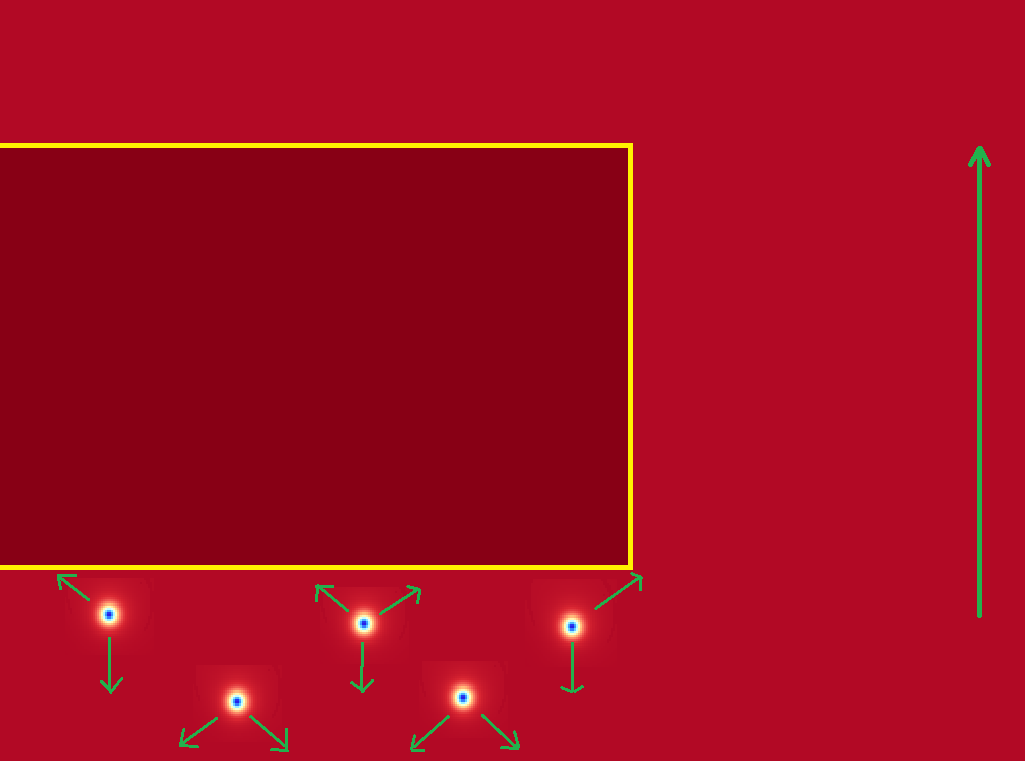
\includegraphics[scale=.50]{forces.png}
\caption{Vortices will be forced in many directions. These can be from the general current, from each other, or from regions of higher $T_c$. Looking at the equation for the order parameter free energy, one can see that it takes more energy to have a vortex in a region of higher $T_c$. The vortex will therefore feel a force away from the boundary with the stronger superconductor (darker red).}
\label{forces}
\end{center}
\end{figure}


\section{Relevant Vortex studies}

Type 2 superconductors, while working at liquid nitrogen temperatures, have the problem of energy dissipation due to vortex dynamics. Therefore many geometric solutions are being worked on to try to slow down this energy loss. Here we focus on two of the most promising, vortex matching and funneling.

\section{Vortex Matching and $\delta T_c$ Pinning}
With improvements in nanotechnology, it has become easier to create grids of inclusions. These can be made by inserting nanorods of different critical superconducting temperature ($T_c$), pulsed laser deposition , by using ion beams to disrupt the superconducting lattice, or by using lithographic techniques.

Inserting nanorods of materials using bulk targets has is benefits and problems. These nanorods can be made to have different $T_c$ by controling the crystalinity or the amount of oxygen doping. \cite{Horii15} found a positive vortex-pinning effect due to the nanorods up to a magnetic field of 5 Tesla. They calculated the inter-vortex distance and designed a particular nanorod density. From there they were able to show that vortex-matching had a stronger pinning effect on the system. Varying the $T_c$ of the system is a powerful way to control the vortex dynamics.

Pulsed laser deposition of YBCO can extend the irreversibility of magnetic fields past the 10 Tesla marker. This was done by using BYTO additions to pin the fluxes. All of this is thanks to the increased availability of ordered nanosized oxide secondary phases in epitaxial thin films. This allows the tuning of material functionalities and has various applications including high temperature superconductors. They observed a large improvement to the critical current compared to untouched YBCO~\cite{Rizzo16}. Accurate placement of inclusions is important as inter-vortex forces are on the order of $1/r$.      

Ion beam etching can also be used to create the necessary inclusions. These antidot arrays can be made on thin films of Niobium Nitride using reactive dc sputtering. The antidot arrays are then created using a mask-aligner to do the ion-beam etching. They find experimental evidence for the observation that the maximum number of vortices which can be captured by an antidot of diameter d is
\begin{eqnarray}
n_s = \frac {d} {4 \xi(t)}, 
\label{}
\end{eqnarray}
where $\xi(t) = \xi_0 / \sqrt{1-t}$ and $t$ is a reduced temperature, typically in the range of $0.9 - 0.95$. They also found that vortices would become trapped in the antidots as well as in the interstices of the antidot lattice. This means that the critical current depends on the geometry of the lattice as well as the direction of current~\cite{Thakur09}. Multiple vortex antidots and inter-vortex trapping are important phenomenta when studying vortex matching. A theoretical basis for vortex matching has also been found. Berdiyorov et. al. ~\cite{Berdiyorov06} used the nonlinear Ginzburg-Landau theory to obtain all configurations for vortices in a grid of defects. They also find that vortices will pin in the inclusions and in between them. For small inclusions, they find only one vortex is trapped per hole. The hole radius and inter-hole distance determines the ability of multiple vortices to be forced into the holes. Like spheres in a box, The vortices prefer a triangular lattice as that affords the densest packing. If the pinning force of the holes becomes small enough, the lattices shift from the grid imposed quadratic lattice to a more natural triangular lattice. They find matching effects at whole and fractional magnatic field to hole ratios. Finally, they found their results to not agree with the Little-Parks theory of superconductors.

Lithographic (sputter etching) techniques were used to create arrays of submicrometere sized pinning arrays. These were compared to simulated $J_c$ curves using the time dependent Ginzburg Landau model. They found that the critical current exibited maxima at the expected matching fields at 2.3 degrees Kelvin. The critical current was considerably larger than systems without antidot arrays~\cite{Sabatino10}.
It is important to have a physical temperature at which these phenomena occur as most Ginzburg-Landau simulations only describe temperature in relation to $T_c$.

\section{Vortex Jamming and Geometric Pinning}
Another way to increase the depinning current of a system is to get the vortices to pin each other. This jamming effect can be accomplished by manipulating the geometry of the system they must past through. Different geometric strategies have been tried including simple funnels, diamonds, and conformal maps. Vortex ratchets and fluxon pumps are also of great interest in the superconducting world. These use diode-like geometries to keep vortices going in one direction. These effects can be seen even with a symmetric force such as an alternating current.  

Computer simulations have been popular in demonstrating the usefulness of vortex ratchets. Within these ratchets, vortices will go through certain phases depending on the strength of the magnetic field. These phases are known as triangular, smectic, disordered, and square~\cite{Lu06}. They showed that sawtooth ridges which modulate the z-component of a superconductor can have a similar effect as triangular modulations in the x and y-components. They used a Langevin model to simulate the vortices, which starts to become unphysical as the vortex density increases.  

The optimal size of the funnel tip is such that only one vortex can pass at a time due to vortex-vortex repulsion forces. Reichhardt et. al.~\cite{Reichhardt10} , through the help of simulations, observed that the sum of the vortex velocities remains constant with increasing magnetic field. They highlight the similarities to a granular hopper, decreasing the width of the hopper aperture decreases the flow of grains. They found that as the number of vortices increases, the pinned vortex structure becomes larger and harder to deform. This then keeps individuals from passing through the bottleneck.

Fluxon pumps can be used to extract useful work from a fluctuating environment. The vortex ratchet can be used as a fluxon rectifier. These could be used as fluxon lenses to concentrate or disperse magnetic fields. These would have various uses including dispersing trapped flux in SQUID magnetometers. But to get the desired effects, the frequency must hit the appropriate resonance region~\cite{Wambaugh99}. This means not only the right frequency for the geometry, but also the correct temperature (i.e. random motion). Thermal noise had to be kept low in the pinning systems. Like sand in an hourglass, minor turbulence has a large effect on the ability of vortices to stick. They again back up the idea that the more fluxons one has, the more their motion will be restricted.

Vortices travelling through constricting lattices can also be used to study the dynamics of interacting particles travelling through confining potentials. Yu et. al. found that with the correct geometry, vortices would begin moving as the external magnetic field varied~\cite{Yu10}. They found strong matching effects between the vortex distribution and the constriction lattice. By tailoring their diamond shaped channel, they could pick their confining potential. The angle of the wall has a strong effect on the ability of the system to be immobilized.

We built upon previous GLGPU research in geometric pinning. In order to simulate geometrical constraints and voids of various shapes we impose appropriate internal boundary conditions or use unstructured grid discretizations~\cite{Kwok16}. The boundary conditions are imposed via picking no current (open) boundaries which simulate insulating inclusions~\cite{Sadovskyy14}. Multiple types of tesselations are also possible, including checkerboard, or less standard Voronoi tesselations. These are useful for polycrystalline thin superconducting films with variations of $T_c$.

\section{GLGPU overview}
GLGPU is a GPU-based Jacobi solver for the time-dependent GL equations. It was designed to solve mesoscale problems which arised in superconductor design. Instead of treating the vortices as elastic strings in a viscous medium, it focuses on the underlying order parameter. This allows for correct interactions between pairs of vortices, vortices and inclusions, and allows the vortices to split up and rejoin. To model the system accurately, we need to take into account the Ginzburg Landau function at a microscopic resolution as a complex valued scalar field. The amplitude of this field is related to the supercondonductivity density, while the phase is related to the current of the system (after a gauge transformation). Through careful optimization, the system size can be made large enough to encompass many vortex interactions and complicated non-superconducting architectures. Physical pinning defects are simulated as modulations of the superconductor's critical temperature. The simulation works by first integrating the GL equations forward in time, then solving the Poisson equiation to find the electric and magnetic fields. There are also noise correlation terms to simulate thermal effects~\cite{Sadovskyy14}.

\subsection{stable GLGPU system}
The particular Ginzburg Landau equations which were used are designed to be particularly stable. In appendix 1, we explore the limits of this system and find it works for all relevant currents. These current equations were :
\begin{eqnarray}
J_N = -\sigma [(1/c) \partial_t A + \nabla \mu ]
\label{currentEq1}
\end{eqnarray}
and
\begin{eqnarray}
J_S = -\frac{e}{2m} [\psi*(i\hbar \nabla + \frac{2e}{c} A) \psi + c.c.],
\label{currentEq2}
\end{eqnarray}
where $\nabla A = 0$, $\sigma$ is the conductivity, $\mu$ is the scalar potential, $A$ is the vector potential, $e$ is electron charge, $c$ is the speed of light, and $m$ is electron mass. To help with stability, the Crank-Nicolson integration scheme and the linearization of the $|\psi|^2\psi$ term were done. An explicit integration would be subject to numerical instabilities.

\subsection{Boundary conditions}

There are two types of boundary conditions relevant to this system. They are quasi-periodic and open. On a quasi-periodic boundary, cells are treated the same as they would be in the middle of the system. The only thing that one needs to keep track of is the phase jump at the boundary. In other words, only the amplitude of the order parameter is really periodic. The open boundary refers to the Neumann boundary conditions. These mean that there is no current perpendicular to the boundary. Specifically;
\begin{eqnarray}
\overrightarrow n (\nabla - i \overrightarrow A)\psi = 0 ,
\lable{}
\end{eqnarray}
where $\overrightarrow n$ is the unit normal vector. For our studies, we stuck with quasi-periodic boundary conditions in the direction of current.



\section{Results}
Being such a general code, there were many possible areas of study regarding this code. We found promissing results in two general areas, grids of inclusions and super conducting-conducting funnels with higher $T_c$. We characterize these situations by looking at their responses to changes in voltage, magnetic field, and geometry. There is an important choice that we made when determining the critical current as there is a inherent hysteresis in the system. We had two options when ramping the current. It could either have been ramped up, Starting with no movement and pushing the current until the vortices became dislodged. The second option was to ramp the current down. That is start with moving vortices and slowly decrease the current until the vortices become lodged. In the end we went for the second option due to the dynamics of the system. Vortices tend to start out placed not according to the lowest energy state, but instead randomly according to whatever starting seed was selected. By forcing the vortices to move around first, we get a more natural state before the depinning current is found. In figure ~\ref{hysteresis} we quantitatively demonstrate the difference.

\begin{figure}[htbp]
\begin{center}
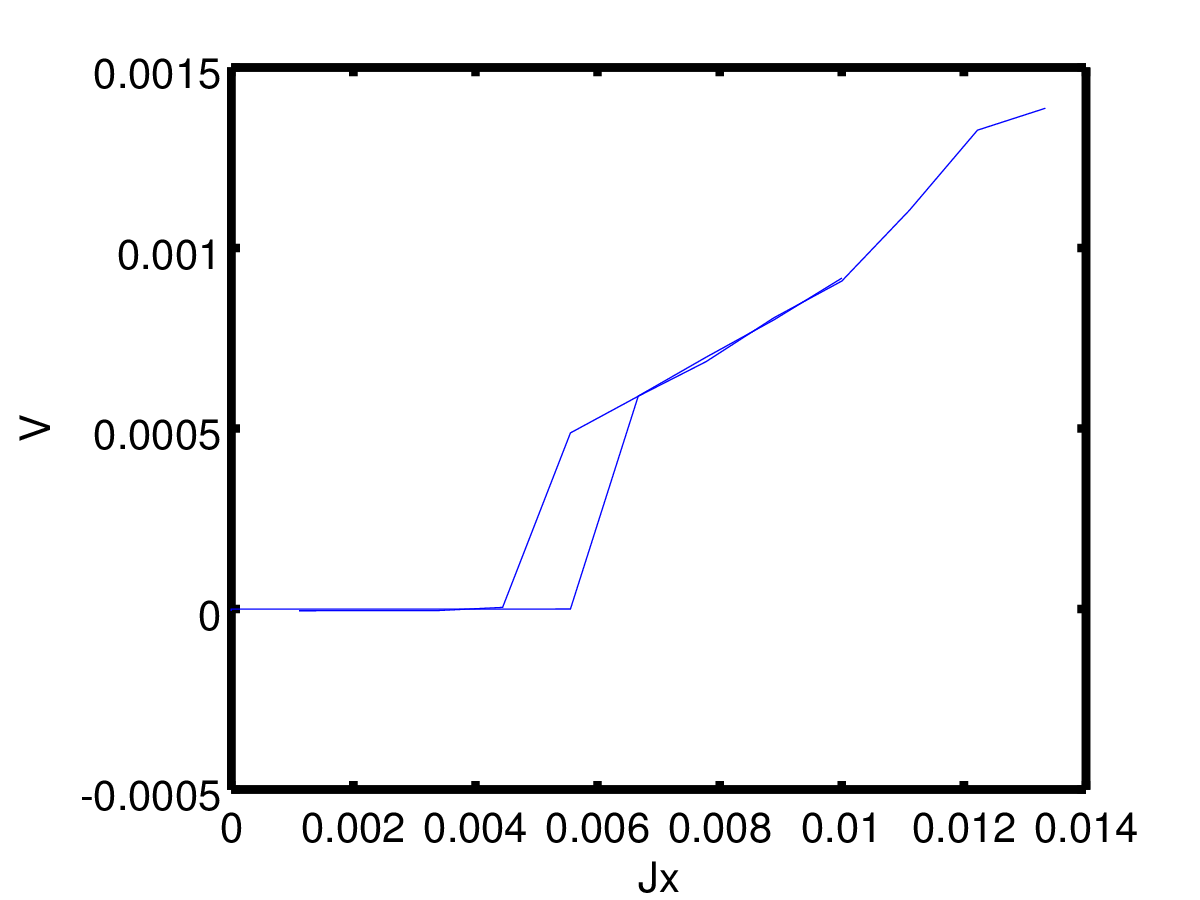
\includegraphics[scale=.50]{Hysteresis.png}
\caption{ Overlapped are the current vs voltage for two systems, one with the current ramped up and one with the current ramped down. Upper one is the current being ramped down, while the lower one is the current ramped up.}
\label{hysteresis}
\end{center}
\end{figure}


\subsection{Grids}
Inclusions in the superconductive substrate can be used to contain vortices (up to a certain current). If these vortices do not move, then they are not draining energy from the system. The first thing we needed to show was that vortices preferred to be trapped in inclusions which were around the same size as they were. If the inclusion size is increased, we see that at some point we start to trap 2 vortices per inclusion. Trapping a vortex requires that the force due to external current and other vortices be less than the superconducting destruction force. The superconducting destruction force is due to the energy of a superconducting system below Tc Being lower than a non-superconducting system below Tc. The second effect we were looking for was vortex matching resistance. Vortices have quantized magnetic flux. This means that for a certain applied field, we can predict the number of vortices. If some vortices are moving and some are pinned, the moving ones will push on the pinned ones as they pass by. If instead we have as many vortices as we have inclusions, after a certain relaxation period, vortices will all be pinned and the system will be more stable. As shown in Fig.~\ref{HDF} we were able to show both of these effects. In the X direction, we see that the optimal radius for an inclusion is 2. In the Y direction, we see a sharp drop in critical current at m=1. This is because as soon as we are above the 1-to-1 ratio, we start to have rogue vortices which will move. As the magnetic field is increased, we start to see that there islands of stability where multiple vortices can fit on the same inclusion. There is also a quadratic relation between the magnetic ratio and the size of the vortices in terms of optimal conditions.

\begin{figure}[htbp]
\begin{center}
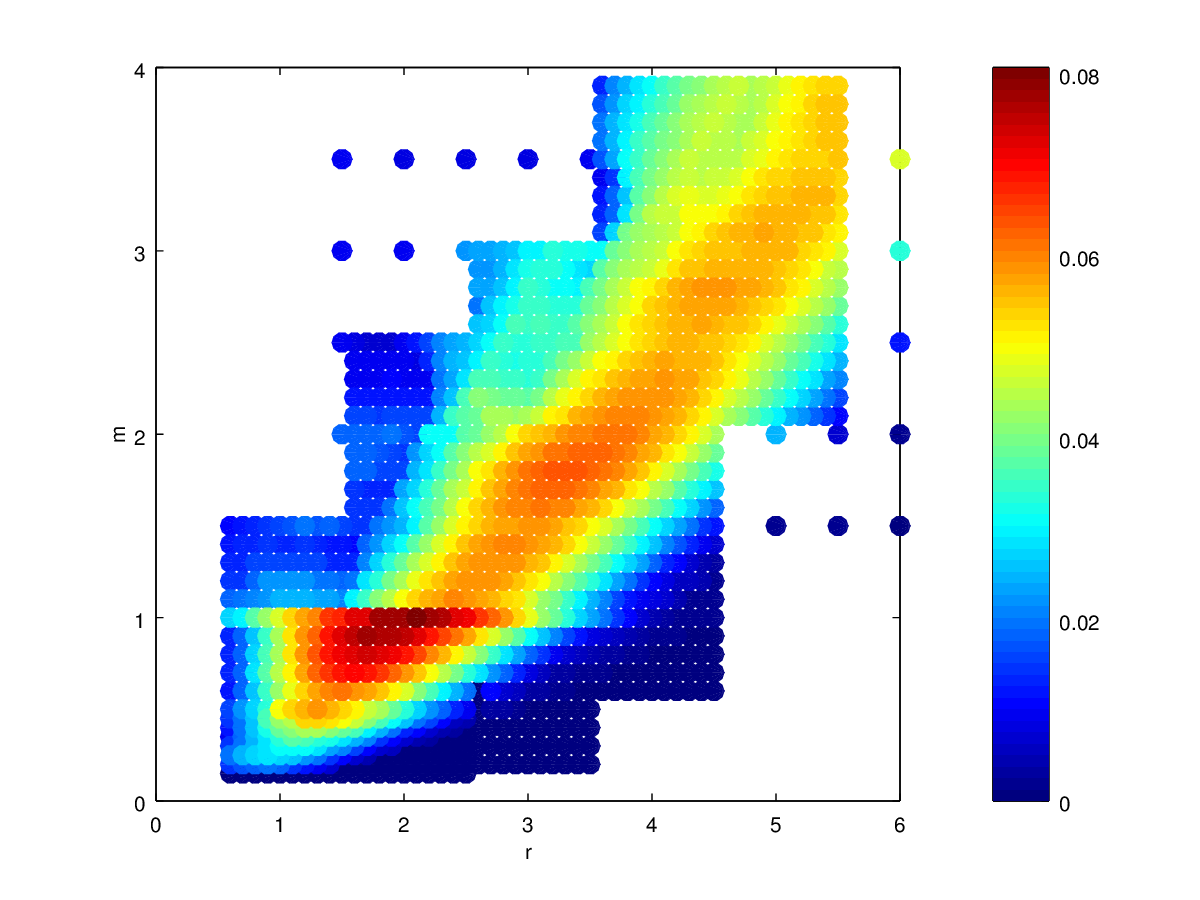
\includegraphics[scale=.50]{HDFinal.png}
\caption{ This is a superposition of 100+ simulations with different parameters. The critical current of each simulation was shown using color. On the X-axis is the radius of each inclusion in the system. On the Y axis m is the ratio of number of vortices per inclusion. The colorbar stands for critical current. In other words, the redder a zone is, the better it holds on to vortices, the higher the current can be before the vortices begin to slip.}
\label{HDF}
\end{center}
\end{figure}

\section{Funnels}
The same way that energy is gained when a vortex goes into a lower superconducting state, energy is lost if it tries to go into a higher superconducting state. Also, since more current can travel through the superconducting system, we get the opposite of the venturi effect. This also helps to keep vortices out. Using this logic, we created superconducting zones with higher $T_c$ that can be used to guide vortices. Indeed, increasing the aperture size increases the ease of which the vortices can travel ~\ref{AvR}.

\subsection{Description}
The magnetic field was kept such that the number of vortices filled 50\% to 80\% of the substrate. It was pointed into the board such that the current pushed the vortices into the funnel. The current was started at an amount large enough to guarantee vortex movement, even if it also meant that vortices went through the walls at first. The current was then slowly relaxed in enough timesteps to make sure that each configuration had enough time to stabilize. The number of current configurations had to balanced against practicallity. Ideally, we would use an infinite number of current configurations, but that would take an infinite ammount of time to simulate. Instead we tried to keep the simulation times at less than 24 hours.

\subsection{Analysis}
In general, the simulations performed as expected. The smaller the aperture, the better a system can hold on to vortices. This is up to a point which where even 1 vortex can no longer slip through. Steeper angles also improved the jamming performance of each system. The dependence did not seem to be linear in y-position of the funnel, or in angle. When looking at the magnetic dependence of the critical current, it is clear that more vortices increase the critical current of the system. In the case of funnel studies, as the angle increases, so does the density of the vortices in the main funnel. That is because the magnetic field was set the same for all runs. As the funnel increases, it takes up more of the main funnel. Still, one can see that the sharper angle has more of a pinning effect even controlling for this effect using the critical current dependence on the magnetic field. 
\begin{figure}[htbp]
\begin{center}
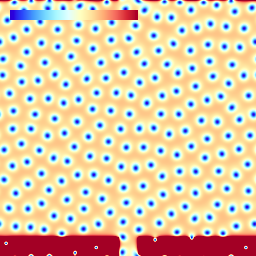
\includegraphics[scale=.50]{ratchetNoAngle.png}
\caption{ The amplitude of the complex order parameter. in yellow is the background superconductor, In red is the superconductor wall, and the blue dots are the vortices. In green is the parameter of interest. In this case, we have a flat obstruction which forces vortices through a narrow gap.}
\label{noAngle}
\end{center}
\end{figure}

\begin{figure}[htbp]
\begin{center}
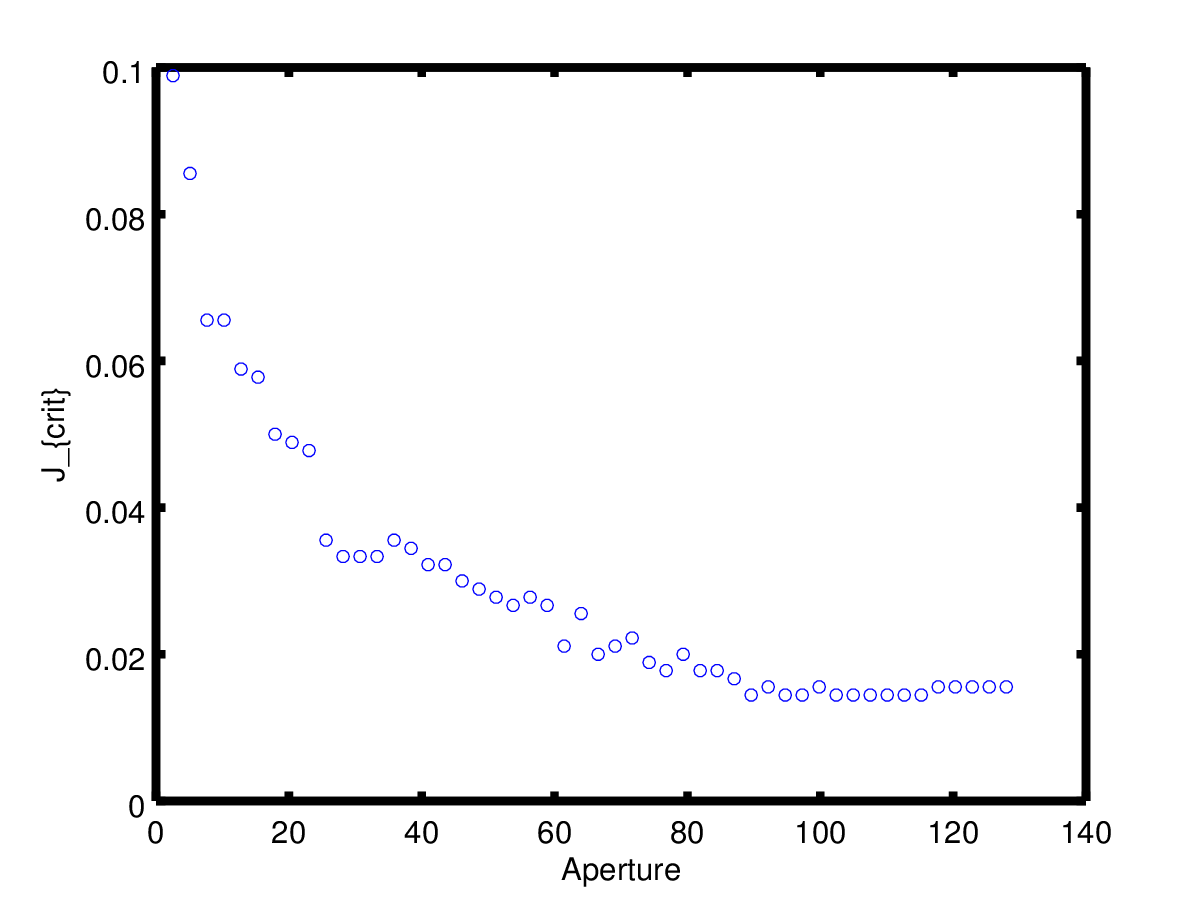
\includegraphics[scale=.50]{flatAperture.png}
\caption{ 50 values of aperture were run in this simulation of a flat system. The resulting current was analyzed to find the critical current . As the aperture is increased, the ability to hold the vortices still is diminished. }
\label{flatScan}
\end{center}
\end{figure}


\begin{figure}[htbp]
\begin{center}
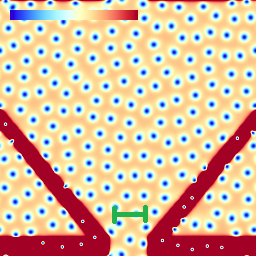
\includegraphics[scale=.50]{normalX.png}
\caption{ The amplitude of the complex order parameter. in yellow is the background superconductor, In red is the superconductor wall, and the blue dots are the vortices. In green is the parameter of interest. In this case it is the size of the aperture which was varied. }
\label{normalX}
\end{center}
\end{figure}

\begin{figure}[htbp]
\begin{center}
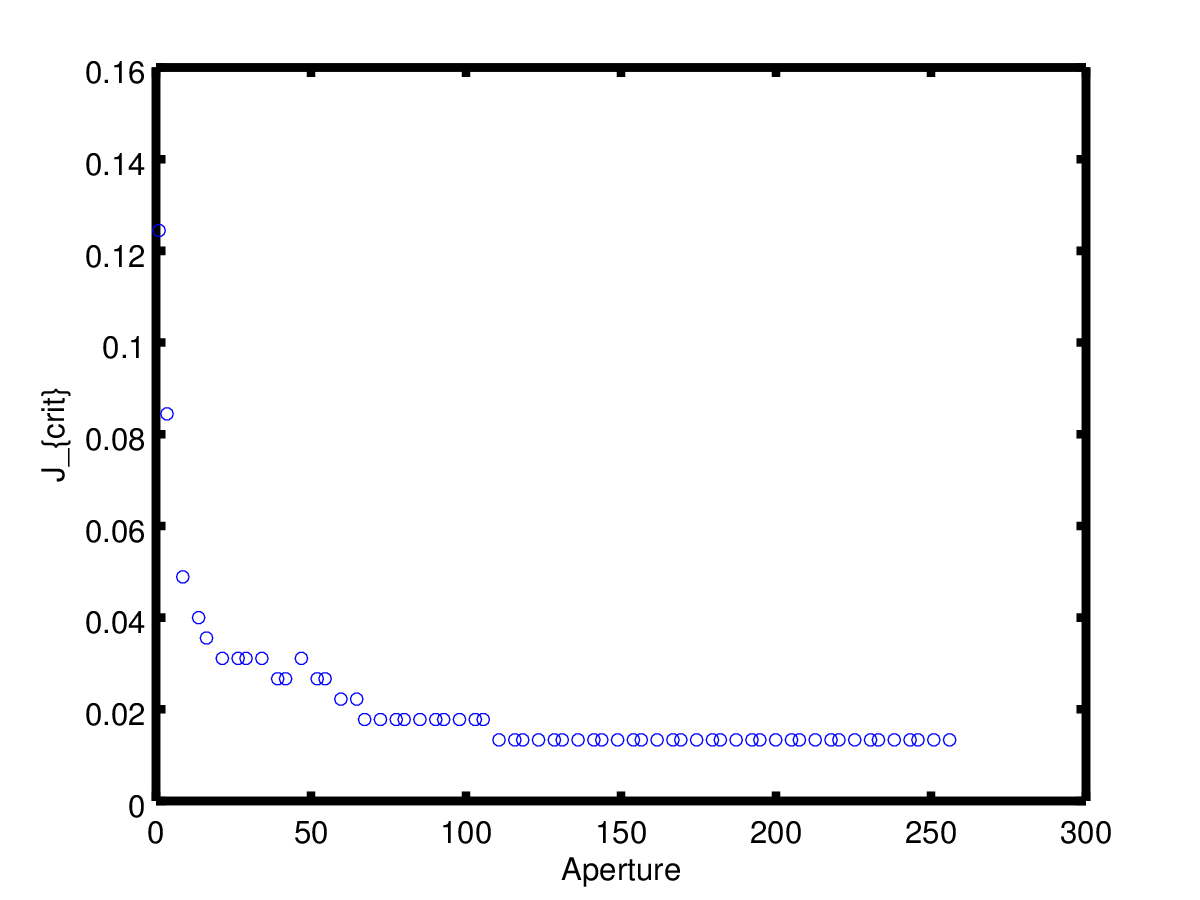
\includegraphics[scale=.50]{funnelX.png}
\caption{ 50 values of aperture were run in this simulation. The resulting current was analyzed to find the critical current . As the aperture is increased, the ability to hold the vortices still is diminished. }
\label{normalXscan}
\end{center}
\end{figure}

\begin{figure}[htbp]
\begin{center}
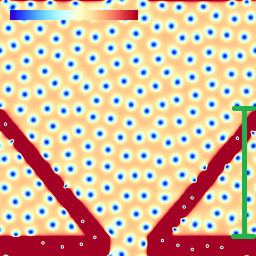
\includegraphics[scale=.50]{normalY.png}
\caption{ The amplitude of the complex order parameter. in yellow is the background superconductor, In red is the superconductor wall, and the blue dots are the vortices. In green is the parameter of interest. In this case it is the point on the Y-axis at which the funnel attaches and therefore the angle which varies. }
\label{normalY}
\end{center}
\end{figure}

\begin{figure}[htbp]
\begin{center}
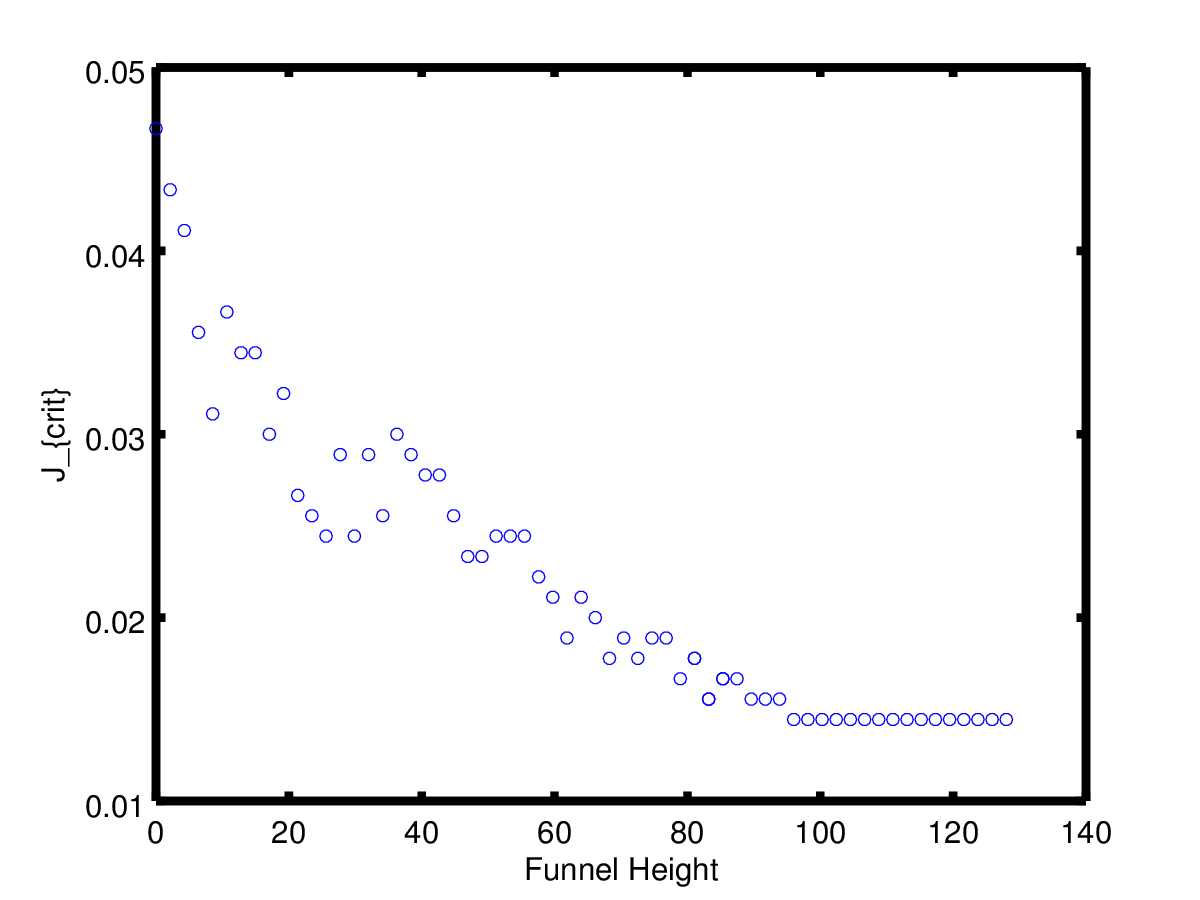
\includegraphics[scale=.50]{funnelY.png}
\caption{ 50 values of aperture were run in this simulation. The resulting current versus voltage information was analyzed to find the critical current . As the angle of the slope is increased, the vortices were more easily jammed. }
\label{normalYscan}
\end{center}
\end{figure}


\begin{figure}[htbp]
\begin{center}
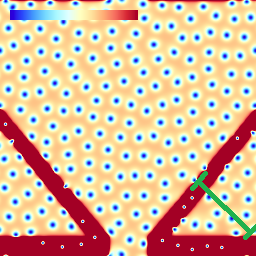
\includegraphics[scale=.50]{normalAngle.png}
\caption{ The amplitude of the complex order parameter. in yellow is the background superconductor, In red is the superconductor wall, and the blue dots are the vortices. In green is the parameter of interest. In this case the angle is held constant while the x and y attachments are varied. }
\label{normalAngle}
\end{center}
\end{figure}

\begin{figure}[htbp]
\begin{center}
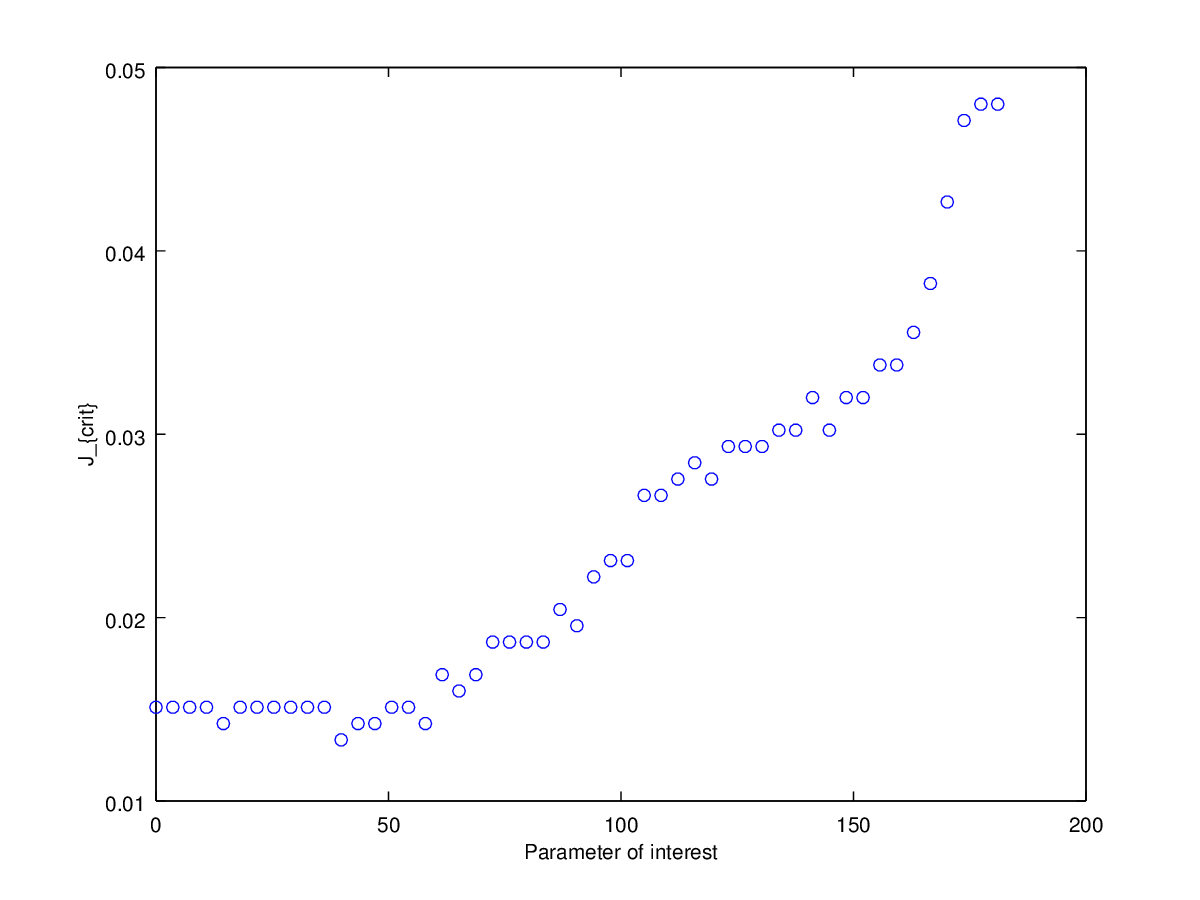
\includegraphics[scale=.50]{constantAngle.png}
\caption{ This is a scan of the parameter of interest versus the critical current. The x-postition and y-position of the funnel were moved uniformly as to keep the angle constant. }
\label{constantAngle}
\end{center}
\end{figure}


\begin{figure}[htbp]
\begin{center}
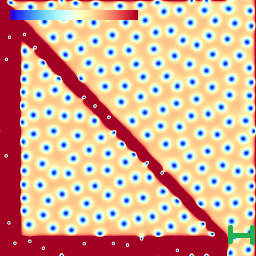
\includegraphics[scale=.50]{oneSidedDone.png}
\caption{ The amplitude of the complex order parameter. in yellow is the background superconductor, In red is the superconductor wall, and the blue dots are the vortices. In green is the parameter of interest. In this case it is the size of the aperture which was varied. }
\label{oneSidedX}
\end{center}
\end{figure}


\begin{figure}[htbp]
\begin{center}
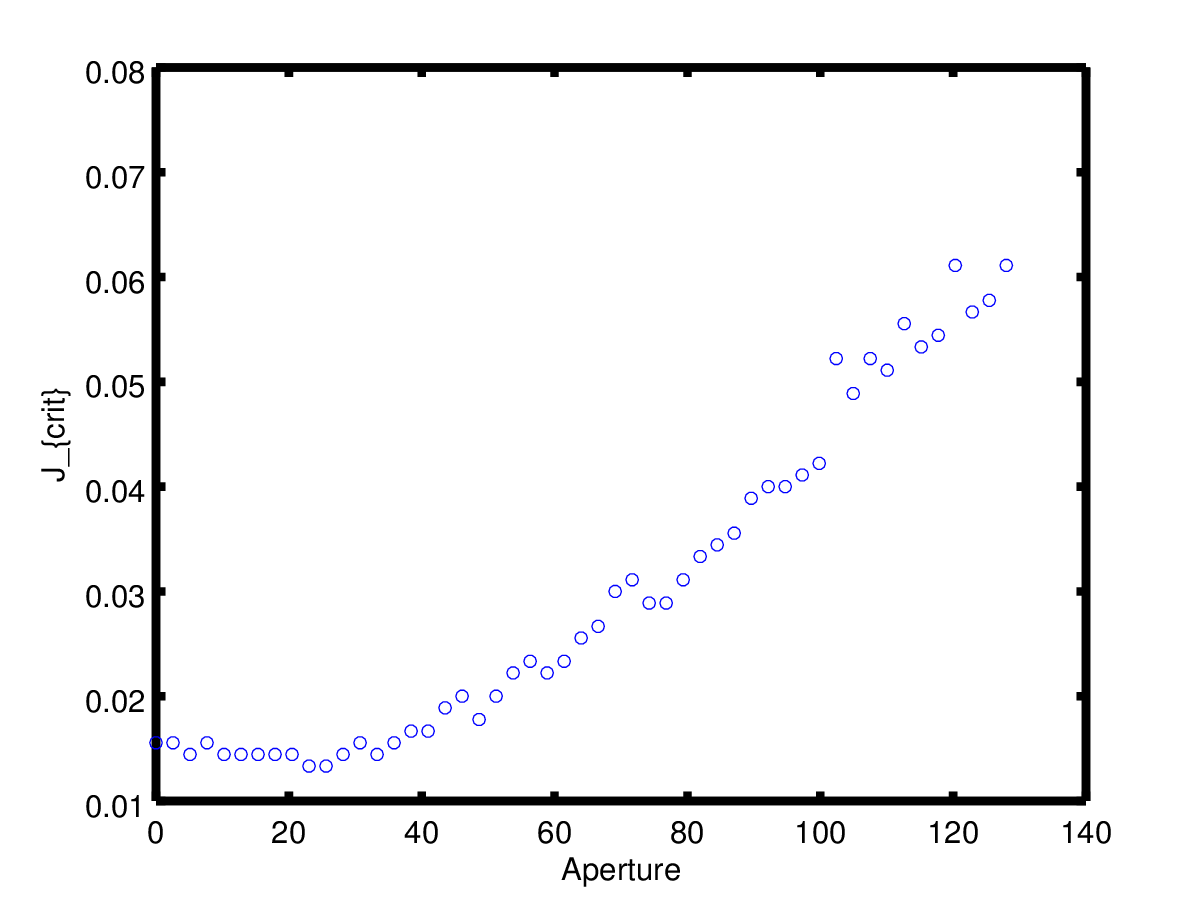
\includegraphics[scale=.50]{oneSideX.png}
\caption{ 50 values of aperture were run in this simulation. The resulting current versus voltage information was analyzed to find the critical current . As the aperture size is increased, the vortices are less restrained. }
\label{normalYscan}
\end{center}
\end{figure}

\begin{figure}[htbp]
\begin{center}
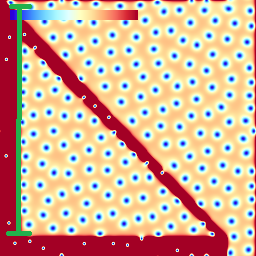
\includegraphics[scale=.50]{oneSidedY.png}
\caption{ The amplitude of the complex order parameter. in yellow is the background superconductor, In red is the superconductor wall, and the blue dots are the vortices. In green is the parameter of interest. In this case it is the point on the Y-axis at which the funnel attaches and therefore the angle which varies.}
\label{oneSidedY}
\end{center}
\end{figure}

\begin{figure}[htbp]
\begin{center}
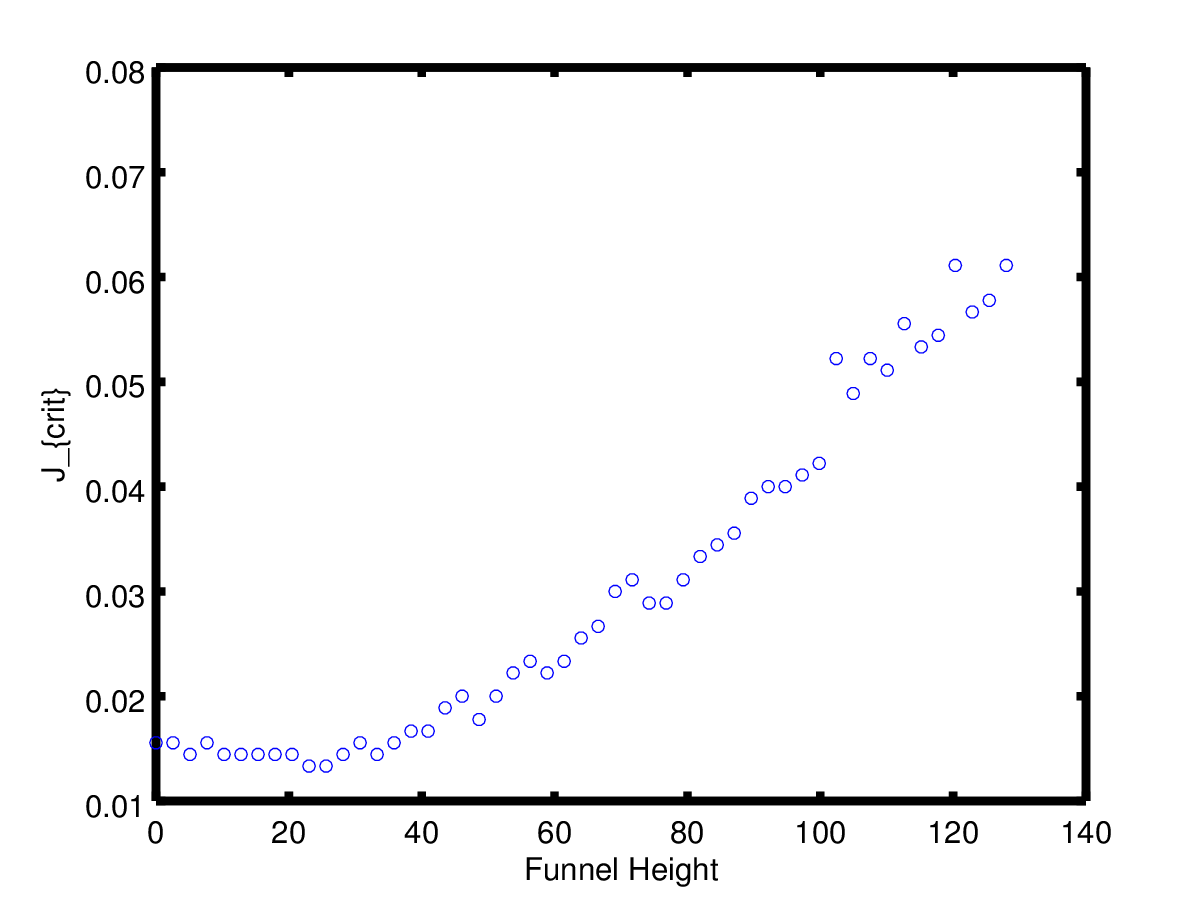
\includegraphics[scale=.50]{oneSideY.png}
\caption{ 50 values of aperture were run in this simulation. The resulting current versus voltage information was analyzed to find the critical current . As the one slope is increased, the jamming effect becomes more pronounced. }
\label{normalYscan}
\end{center}
\end{figure}


\begin{figure}[htbp]
\begin{center}
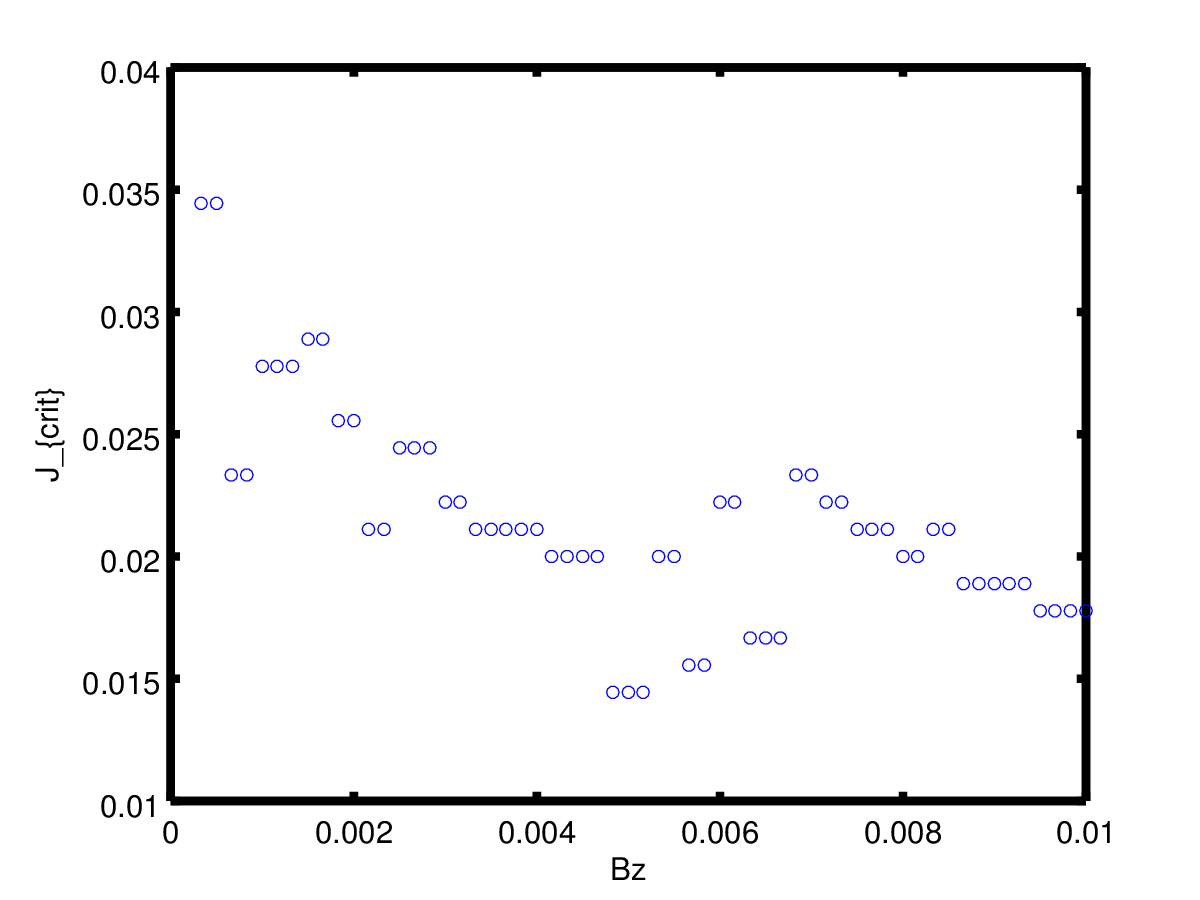
\includegraphics[scale=.50]{2DAngleBz.png}
\caption{ 50 values of the magnetic field angled system. The resulting current versus voltage information was analyzed to find the critical current .  }
\label{angleBz}
\end{center}
\end{figure}


\begin{figure}[htbp]
\begin{center}
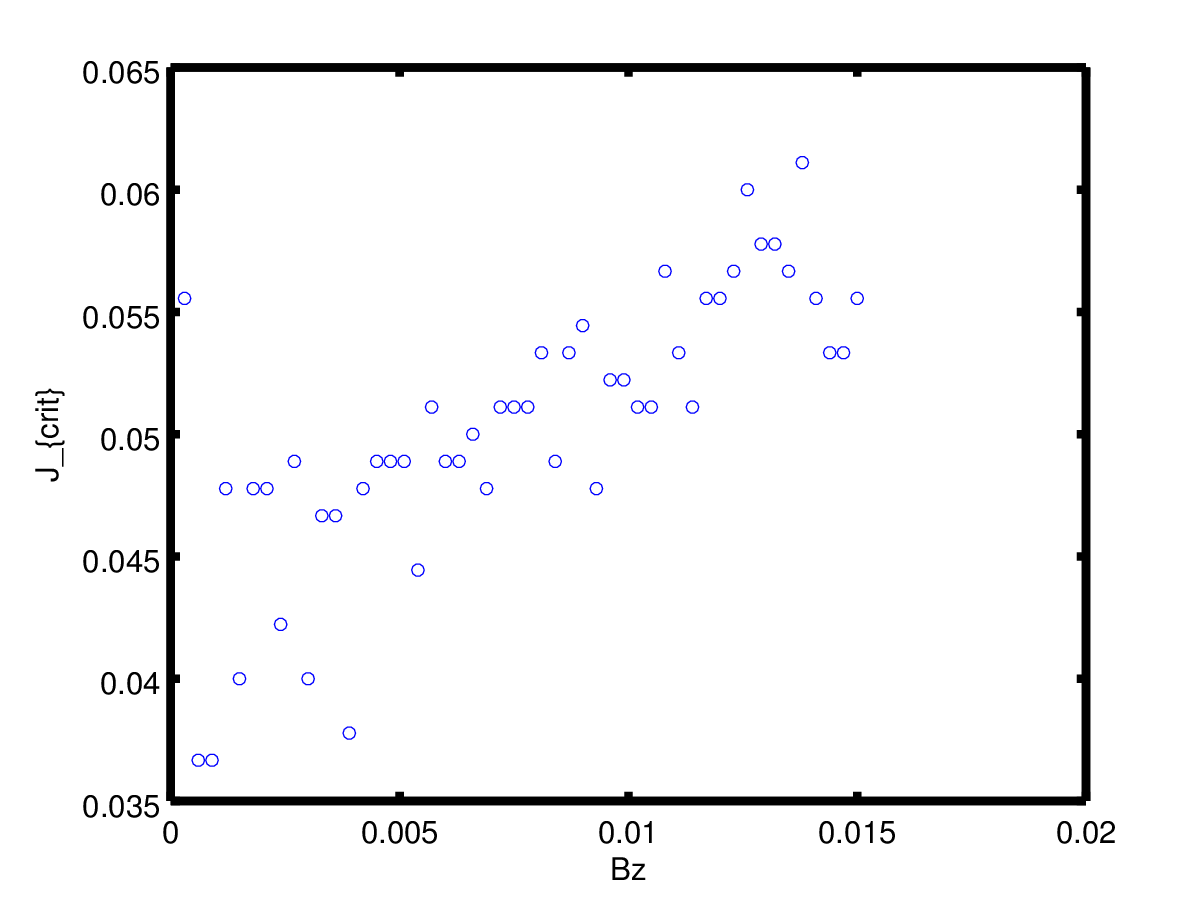
\includegraphics[scale=.50]{emptyDiamondBz.png}
\caption{ 50 values of the magnetic field were studied for the empty diamond system. The resulting current versus voltage information was analyzed to find the critical current .  }
\label{emptyBz}
\end{center}
\end{figure}

\begin{figure}[htbp]
\begin{center}
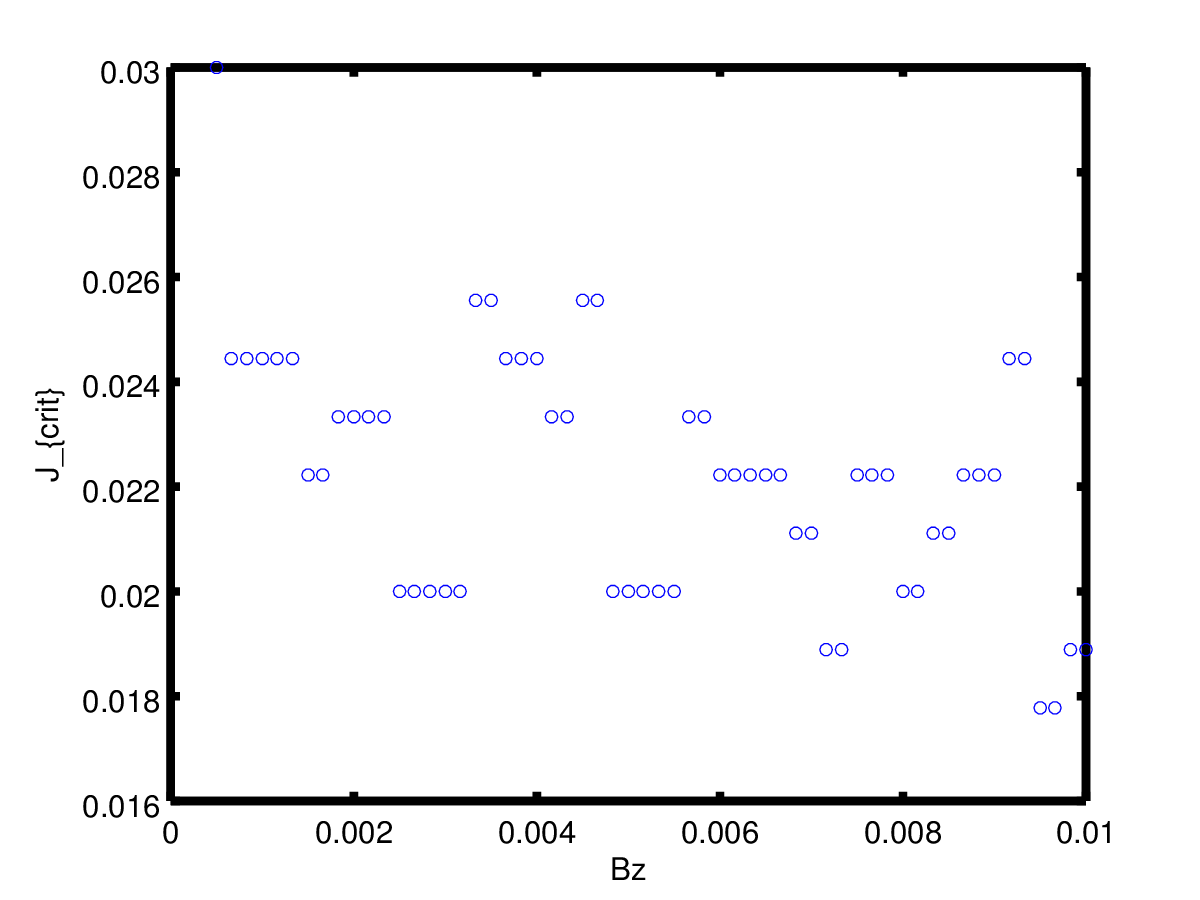
\includegraphics[scale=.50]{2DFlatBz.png}
\caption{ 50 values of the magnetic field were studied for the flat system. The resulting current versus voltage information was analyzed to find the critical current .  }
\label{flatBz}
\end{center}
\end{figure}

\begin{figure}[htbp]
\begin{center}
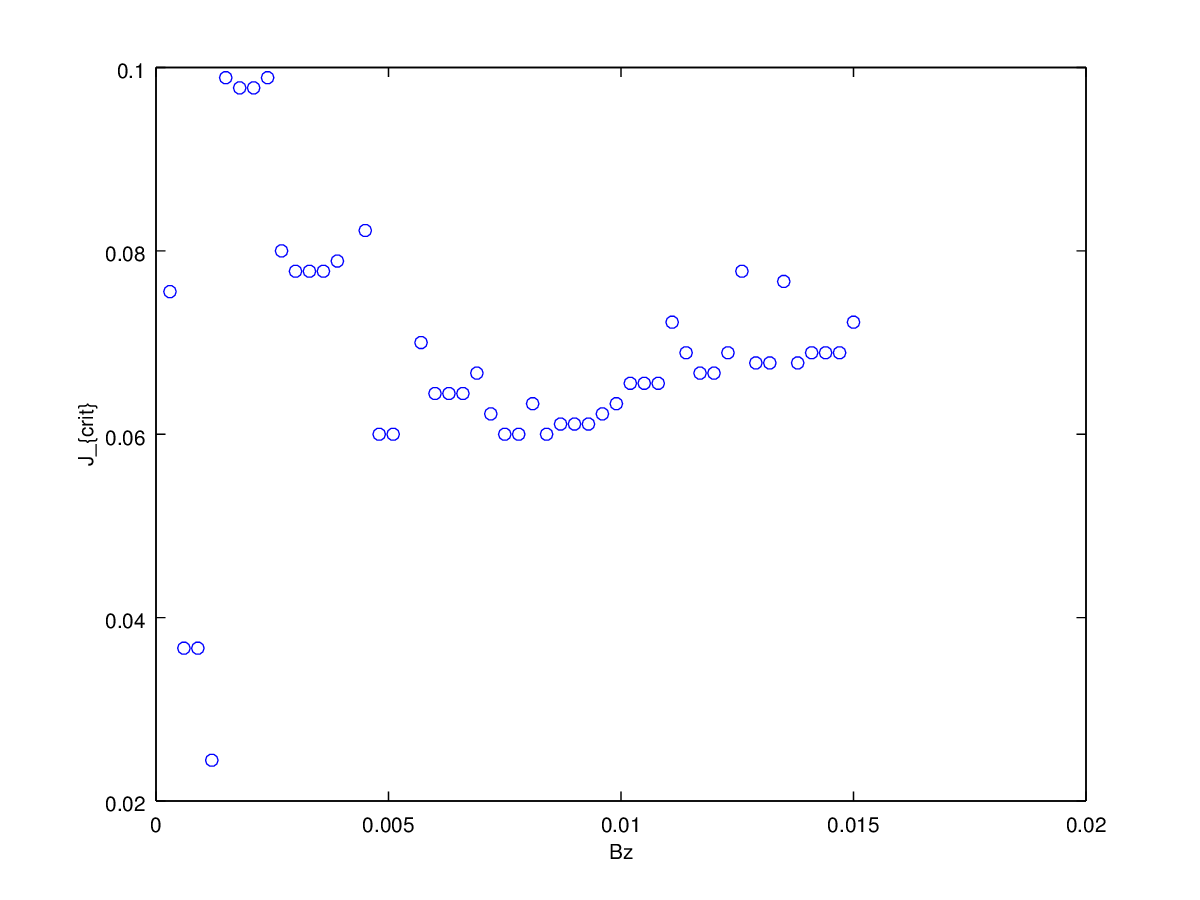
\includegraphics[scale=.50]{oneSideBz.png}
\caption{ 50 values of the magnetic field for the one sided system. The resulting current versus voltage information was analyzed to find the critical current .  }
\label{oneBz}
\end{center}
\end{figure}

To conclude, we have explored multiple systems with the use of the GL program. We showed that if the number of inclusions matches the number of vortices, the system jams and we have much lower resistance due to vortex motion. We have also explored many funnel systems which are currently being tried out experimentally throughout the superconduction community. We showed that vortex jamming is a function of the angle of the funn
el, the size of the aperture, and the amount of vortices.

 
